\subsection{What identifiability
means}\label{what-identifiability-means}

At a general level, write \(\Theta_P=\{\theta:P_\theta=P\}\) for the
observational equivalence class of latent structures that produce the
same observed distribution, and let \(\mathcal G\) denote the model's
symmetry group, which includes permutations of the environment labels
and any other parameterization symmetries. The structure is identifiable
up to \(\mathcal G\) when every member of \(\Theta_P\) is a
\(\mathcal G\)-image of the others. Below we use the concrete
decomposition-set version of this class, restricted to mixtures over
component laws.

Let \(P_X\) be the pooled marginal, and write a mixture as a measure
over component laws, \(\mu=\sum_e a_e\delta_{G_e}\), with \(a_e>0\) and
\(\sum_e a_e G_e=P_X\). The decomposition set is

\begin{equation}\label{eq:identified-set}
\mathcal D(P_X)=\left\{\mu=\sum_e a_e\delta_{G_e}:\ a_e>0,\ \sum_e a_e G_e=P_X\right\}.
\end{equation}

The structure is identified up to label permutation when
\(\mathcal D(P_X)\) is a singleton. With only \(P_X\) in hand, the joint
law of \((X,E)\) is not fixed. Any Markov kernel \(\kappa(e\mid x)\)
whose integral against \(P_X\) matches the label marginal is a valid
assignment, and outside degenerate cases the set of such kernels
contains more than one point. The next result makes this concrete with
an explicit witness.

\subsection{Partition
non-identification}\label{partition-non-identification}

\begin{theorem}[the pooled marginal does not determine the partition]\label{thm:d2}
There exist two environment assignments $\sigma$ and $\sigma'$, not related by a global label permutation, that hold simultaneously under one and the same observation distribution. A measure-preserving bijection $T$ on the latent space satisfies
\begin{equation}\label{eq:witness}
T_\#P_Z=P_Z,\qquad \sigma'=\sigma\circ T,\qquad \sigma'\notin\{\sigma,\ 1-\sigma\}.
\end{equation}
\end{theorem}

The scope is deliberately narrow. The statement concerns the class of
assignments that carry no structural constraint: when the assignment is
free to be any measurable partition, the pooled marginal cannot identify
the sample-level partition. It does not say a partition is
non-identifiable once the component laws are restricted to a structured
family, the case taken up below.

\emph{Proof sketch.} On the unit disk, the quarter turn
\(T(z_1,z_2)=(-z_2,z_1)\) preserves the uniform measure, so the two
assignments, split by the first and by the second coordinate
respectively, induce the same pooled distribution yet disagree on the
first and third quadrants with probability \(1/2\), which a label
permutation cannot produce. The full construction is in Appendix A.2.
Figure~\ref{fig:witness} depicts the two assignments and
the disagreement region.

\begin{figure}[htbp]
\centering
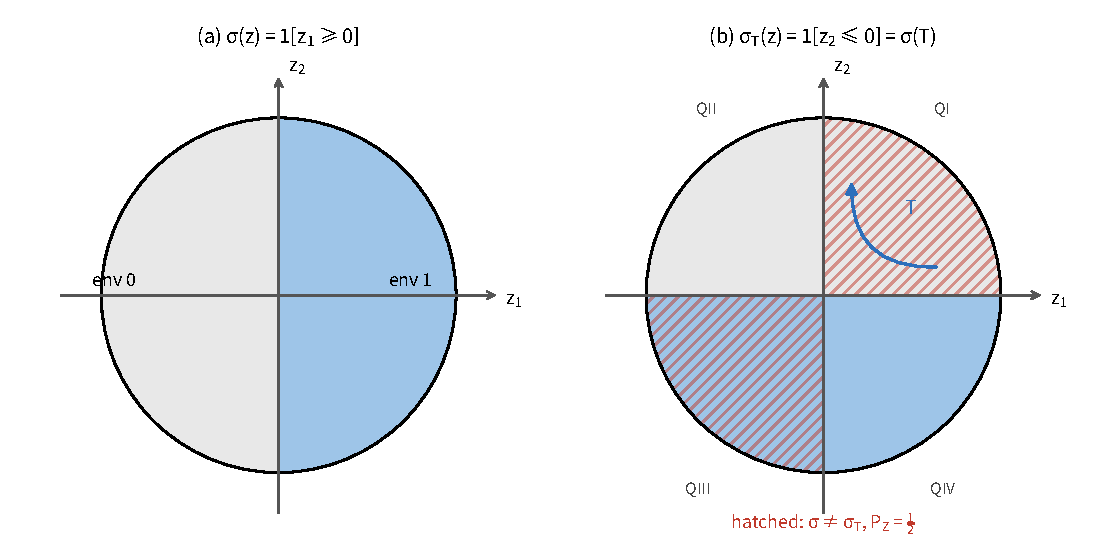
\includegraphics[width=0.92\columnwidth]{fig5_witness.pdf}
\caption{The $d=2$ non-identification witness. Left: the assignment $\sigma=\mathbb 1[z_1\ge0]$ splits the disk by the first coordinate. Right: the rotated assignment $\sigma'=\sigma\circ T=\mathbb 1[z_2\le0]$; the hatched first and third quadrants are where the two disagree, with total probability $1/2$, while the quarter turn leaves the pooled distribution unchanged.}
\label{fig:witness}
\end{figure}

On \(2\times10^5\) draws the disagreement fraction is \(0.5000\), and
the squared maximum-mean-discrepancy between \(Z\) and \(T(Z)\) is
\(0.00058\), finite-sample noise around a population value of zero. This
is a single \(d=2\) witness on the class of arbitrary measurable
assignments, not a claim that every pooled distribution is
non-identifiable, and the witness need not remain inside a smaller
structured class.

The component laws in the witness are not Gaussian. Each environment is
uniform on a half-disk, a bounded-support law with mean
\(4/(3\pi)\approx 0.424\) along the symmetry axis and covariance
approximately \(\mathrm{diag}(0.070,0.250)\). The construction therefore
lives in the broad class of bounded-support models, not the parametric
Gaussian class used later, and the freedom it exploits is freedom in the
component laws themselves, which a fixed parametric family removes.
Classical finite-mixture identifiability, in the form of
Teicher~\cite{teicher1963}, states that a Gaussian
mixture with a known number of distinct components is identifiable up to
a label permutation, so two genuinely different Gaussian partitions with
one pooled law cannot be constructed. That is exactly why the
constrained model in the next section reaches point identification.

A second, covariance-level example illustrates the same limitation
within a Gaussian setting. Consider two zero-mean two-component Gaussian
models with equal weights. In the first the component covariances are
\(\Sigma_1=\mathrm{diag}(1,3)\) and \(\Sigma_2=\mathrm{diag}(3,1)\); in
the second they are \(\Sigma_1'=\Sigma_2'=\mathrm{diag}(2,2)\). Both
induce the same pooled covariance, \(\mathrm{diag}(2,2)\), yet the
component structures differ and the full distributions are not the same.
A single pooled second moment is a many-to-one summary, so it cannot
recover the assignment. The full distribution of a fixed Gaussian family
can, up to permutation, and that distinction is the boundary between the
present witness and the point-identification result that follows.

\subsection{Point identification in a symmetric two-component
covariance-mixture
model}\label{point-identification-in-a-symmetric-two-component-covariance-mixture-model}

Tighten the setting and the decomposition set collapses to a point. Let
\(E\in\{+1,-1\}\) carry equal weight, with zero-mean Gaussian components

\[X\mid E=+1\sim N(0,I+K),\qquad X\mid E=-1\sim N(0,I-K),\]

where \(K\) is symmetric and every eigenvalue of \(K\) lies strictly
inside \((-1,1)\). The pooled covariance is \(I\), so the frame is
whitened. The object identified is the unordered component covariance
pair \(\{I+K,I-K\}\), not the pooled covariance and not any recording
assignment. The result is a special fourth-moment inversion: with the
second moment fixed by whitening, the fourth-order cumulant tensor is
inverted algebraically to recover the pair.

\begin{theorem}[point identification of the component covariance pair]\label{thm:pointid}
In the symmetric two-component model above, the fourth-order cumulant tensor determines $K$ up to the global sign $K\leftrightarrow-K$ in $d=2$, and hence determines the unordered component covariance pair uniquely. Write $K=Q\operatorname{diag}(\lambda_1,\lambda_2)Q^\top$. The following cases are exhaustive.

\textbf{Case (i): $\lambda_1^2\ne\lambda_2^2$.} The contraction $T$ has two distinct eigenvalues, and diagonalizing it recovers the eigenbasis; the eigenvalue magnitudes and their relative sign follow from the diagonal cumulants.

\textbf{Case (ii): $\lambda_1=-\lambda_2\ne0$, so $\operatorname{tr}K=0$ and $T$ is scalar.} The entries of $K$ are recovered directly from the full tensor by the algebraic identities~\eqref{eq:direct-recover}, with no ratio and no singular direction; the swap configuration $K_{11}=0$ is included.

\textbf{Case (iii): $\lambda_1=\lambda_2\ne0$, so $K=\lambda_1 I$ is isotropic.} There is no basis to recover, and the single value follows from $\kappa_{1111}/3$.

\textbf{Case (iv): $\lambda_1=\lambda_2=0$, so $K=0$.} The zero cumulant tensor forces $K=0$ uniquely, but the two component covariances coincide at $I$; two distinct components and an eigenbasis are not identified.

The only genuine observational freedom is the global sign $K\leftrightarrow-K$, which is exactly the label permutation exchanging $I+K$ with $I-K$.
\end{theorem}

\emph{Proof sketch.} The pooled fourth cumulant is
\(\kappa_{ijkl}=K_{ij}K_{kl}+K_{ik}K_{jl}+K_{il}K_{jk}\). Contracting
the middle indices gives a matrix that commutes with \(K\) and, whenever
it is non-scalar, reveals the eigenbasis, after which the diagonal
cumulants fix the magnitudes and the relative sign; the scalar,
isotropic, and zero cases follow from the algebraic
identities~\eqref{eq:direct-recover} and
\(\kappa_{1111}/3\). The full derivation, including the swap
configuration and the sign recovery, is in Appendix A.1.

The same tensor structure appears in higher dimensions, where locating
the eigenbasis is a symmetric tensor decomposition, but we do not prove
that extension and the formal theorem is stated for \(d=2\). The generic
map for centered Gaussian mixtures is non-injective at fourth order and
reaches injectivity at sixth order, as discussed in Chapter 2 and the
finite-moment literature cited there. Whitening, the two-component
restriction, equal weights, and symmetry are the conditions that yield
injectivity, so this is not a generic fourth-order theorem.

The whitening is a population condition. The theorem assumes the pooled
covariance is exactly \(I\), so the whitening is population-known.
Estimating it from a finite sample introduces sampling error and the
cumulant inversion would then be approximate, and a finite-sample
theorem with estimated whitening is not established here. The result is
a population statement on an idealized Gaussian frame and has no direct
applicability to the empirical EEG covariance features, which are
estimated and not whitened in this model.

Two terms should be kept apart. The theorem identifies the unordered
covariance pair, which can collapse to a singleton when \(K=0\), as in
Case (iv); it does not identify two distinct environments in that
degenerate case, which require \(K\ne0\). Neither case identifies
recording-level labels, which lie outside the scope of the theorem.

\subsection{Scope}\label{scope-4}

These results operate on one pooled marginal and identify either the
partition witness or the unordered component parameters. They do not
identify recording assignments, establish finite-sample recovery, or
support the DELVE algorithm in Section 5. No implication runs from one
mechanism to the other, and the generic non-Gaussian, fully blind
identification problem remains open and is stated in the limitations.
